\documentclass{article}
%\title{LTC Reader Owner's Manual}\label{ltc-reader-owners-manual}
\title{\textbf{LTC Reader Owner's Manual}}
\date{} % Устанавливаем пустую дату
\author{}


\usepackage[a4paper, left=2cm, right=2cm, top=2cm, bottom=2cm]{geometry}
%\usepackage{hyperref} % Загружаем пакет для гиперссылок
\usepackage{graphicx}
\usepackage{enumitem} % Подключаем пакет для работы со списками
\usepackage{longtable} % Подключаем пакет для длинных таблиц
\usepackage{booktabs}  % Подключаем пакет для красивых таблиц
\usepackage{tabularx}  % Для управления шириной столбцов
\usepackage{fancyhdr} % Для пользовательских колонтитулов
\usepackage{float}
\usepackage{tcolorbox} % для callout
\usepackage{mdframed} % для callout
\usepackage{fontspec}

\usepackage[hidelinks]{hyperref} % Убрать цветные рамки вокруг ссылок

% Устанавливаем шрифт Open Sans
\setmainfont{Open Sans}


% Переопределяем команды для заголовка
%\renewcommand{\title}[1]{\begin{center}\textbf{\huge #1}\end{center}}
%\renewcommand{\author}[1]{\begin{center}\textbf{#1}\end{center}}
%\renewcommand{\date}[1]{\begin{center}\textbf{#1}\end{center}}

\begin{document}

	\begin{titlepage} % Титульный лист
		\centering
		\maketitle
		\thispagestyle{empty} % Убирает номер страницы на первой странице
		\vspace{1cm} % Отступ перед изображением
		\begin{figure}[h]
			\centering
			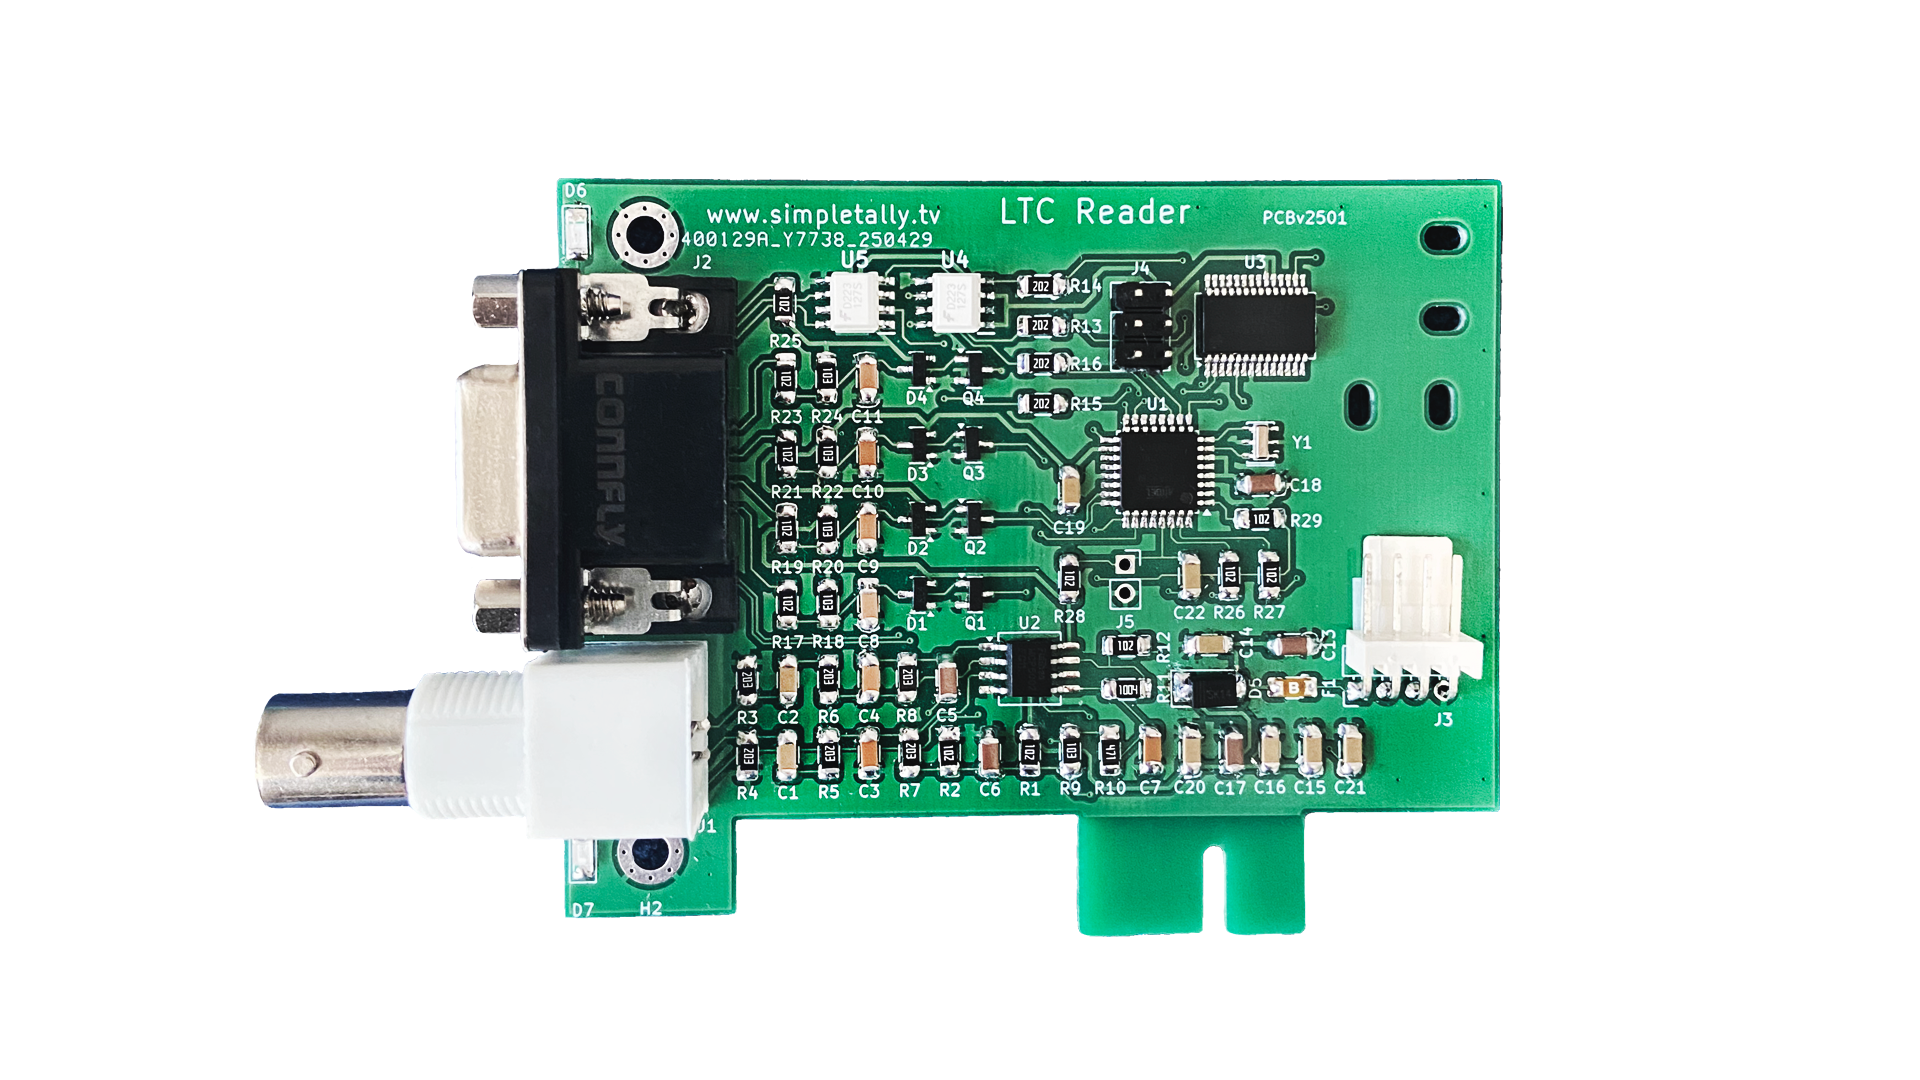
\includegraphics[width=\textwidth, keepaspectratio]{imgs/schema.png}
		\end{figure}
		\vfill % Отодвигает текст вниз страницы
		% Текст внизу страницы
		\Large
		May 2025 \\
		SimpleTally \\
		\href{http://www.simpletally.tv}{www.simpletally.tv}
	\end{titlepage}
	\pagenumbering{arabic} % Устанавливает арабскую нумерацию
	\setcounter{page}{2}   % Устанавливает номер страницы на 1 для следующей страницы	
	\tableofcontents % Вставка оглавления
	\newpage % Переход на новую страницу после оглавления
	
	\section{About}\label{about}
		\noindent LTC Reader, hereinafter referred to as the Device, is used to:
		\begin{itemize}
			\item
			 synchronize a computer or server from the LTC signal
			\item
			receive 4 GPI input signals
			\item
			send 4 GPI output signals
		\end{itemize}
		\noindent Supported OS:
		\begin{itemize}
			\item
			Windows
			\item
			Linux
		\end{itemize}
	
	\section{LTC Reader Basics}\label{ltc-reader-basics}
		\subsection{Basic connection}\label{basic-connection}
			The basic functional connection for Device consists of:
			\begin{itemize}
				\item 1 x Linear Time Code (LTC) input
				\item 1 x USB 2.0 communication port of a computer
				\item 4 x General Purpose Interface Input
				\item 4 x General Purpose Interface Output
			\end{itemize}
	
		\subsection{Connection to computer or server}\label{connection-to-computer-or-server}
			\begin{enumerate}
				\item Place Device in PCI or PCIe x1-x16 slot.
				\item Connect cable to connector J3 on Device and USB2.0 connector at
				computer.
			\end{enumerate}
			\begin{quote}
				The slot serves only for the mechanical placement of the board. Data and 	power are transmitted via USB HU-4 cable through the J3 connector on the board.
			\end{quote}
			\begin{quote}
				It is possible to connect Device to PLS-4 connector on motherboard using a special cable, which is purchased separately. Attention, it is important not to confuse the polarity when connecting. Improper connection can cause the device or motherboard fatal damage.
			\end{quote}
	
		\subsection{LTC Input}\label{ltc-input}
			The input accepts a Linear Time Code (LTC) signal from either a balanced or unbalanced source. The shell of the BNC input connector is floating above ground. For an unbalanced source connect the input using a standard BNC-BNC or a BNC-Phono cable. For a balanced source leave the cable shield unconnected at the LTC Reader end and connect the balanced signal between the center pin and the shell of the BNC connector.
	
		\subsection{USB 2.0 connection}\label{usb-2.0-connection}
			The LTC Reader is designed for direct connection to	
			\begin{itemize}
				\item
				a PC computer's standard USB 2.0 port
				\item
				4-Pin plug 2.54 mm (PLS-4 or DS-1021-1x4)
			\end{itemize}
			Power is derived from USB 2.0 port.
	
		\subsection{General Purpose Interface (GPI) Connector}\label{general-purpose-interface-gpi-connector}
			A 15 pin high density D-Sub socket connector (DHR-15FB / DS1038-15F) on the side of the LTC Reader is used for both GPI inputs and outputs. A 15 pin high density D-Sub plug connector (DS1035-15M) is supplied with the unit for termination by the customer.
	
		\subsubsection{GPI Outputs}\label{gpi-outputs}
			\paragraph{}
				There are four opto-isolated outputs on the LTC Reader. Each output is a NPN transistor with the emitters connected to common pin. The operation of each of the GPI outputs is software programmable to operate under direct software control.
	
		\subsubsection{GPI Inputs}\label{gpi-inputs}
			\paragraph{}
				There are four GPI inputs. These inputs are protected by clamping diodes 	and current limiting series resistors. The inputs are pulled up internally to logic Vcc and may be operated by a pull down to logic ground. The common logic ground is connected to the frame ground of the communications port. Each of the GPI inputs may be programmed to transmit a serial report to 	the Computer's Virtual Com port. This may be displayed by the host software on the computer or may be used to initiate another action.
		
		\subsubsection{GPI pinout}\label{gpi-pinout}
			\begin{center}
				\begin{tabular}{|c|c|}
					\hline
					Pin number & Signal \\
					\hline
					01 & GPI-1 \\
					02 & GPI-2 \\
					03 & GPI-3 \\
					04 & GPI-4 \\
					05 & NC \\
					06 & GND \\
					07 & GND \\
					08 & GND \\
					09 & GND \\
					10 & GND \\
					11 & GPO-1 \\
					12 & GPO-2 \\
					13 & GPO-3 \\
					14 & GPO-4 \\
					15 & NC \\
					\hline
				\end{tabular}
			\end{center}
	
		\subsection{Status LED}\label{status-led}
			There are two LEDs:
			\begin{center}
				\begin{tabular}{|c|c|c|c|}
					\hline
					\# & Color & Position & Value \\
					\hline
					1 & Red & Near D-Sub connector & Power on \\
					2 & Green & Near BNC connector & LTC input valid \\
					\hline
				\end{tabular}
			\end{center}
	
	\section{Serial communications protocol}\label{serial-communications-protocol}

		\subsection{Serial Communications Protocol}\label{serial-communications-protocol-1}
			Control of the LTC Reader is by a simple string of ISO characters. Control strings and User Group hexadecimal digits are case sensitive and \textbf{must} be entered as upper case characters. Commands, except control character commands, are terminated with a carriage return character (0D hex).
			LTC Reader responds to valid commands that require a data response with a data report. All other commands are acknowledged by:
			\begin{center}
				\begin{tabular}{|c|c|}
					\hline
					Acknowledge & Value \\
					\hline
					OK & for valid commands \\ 
					NA & for commands which are temporarily disabled by another function \\ 
					NV & for not valid commands \\
					\hline  
				\end{tabular}
			\end{center}
			All responses are terminated with a carriage return character.
			The serial port operates at:
		\begin{itemize}
			\item
			19200 baud
			\item
			8 data bits
			\item
			no parity
			\item
			1 stop bit.
		\end{itemize}
		For continuous reporting of a maximum length report at 30 frames per second there is about 12\% idle time left between reports.
		
	\subsection{Data Report Format for Time Address, User Groups \& Status.}\label{data-report-format-for-time-address-user-groups-status.}
		The output preset data report format may consist of up to three blocks of data:
		\begin{itemize}
			\item
			The Time Address
			\item
			User Groups
			\item
			Status blocks
		\end{itemize}
		Any data block may be individually enabled or disabled. The blocks are separated by single space characters. The Time Address and User Groups may also be formatted without separator characters for faster transmission or with separator characters for legibility when sent directly to a screen or printer.	
		\begin{center}
			\begin{tabular}{|c|c|}
				\hline
	       		Command & Value \\
				\hline
	       		RF\textgreater1 & PRINT format. \textbf{HH:MM:SS;FF hh.hh.hh.hh sfftt} \\ 
				RF\textgreater0 & Unformatted. \textbf{HHMMSSFF hhhhhhhh sfftt} \\ 
				RT\textgreater0 & Exclude Time Address from report \\ 
				RT\textgreater1 & Include Time Address with report \\ 
				RU\textgreater0 & Exclude User Groups from report \\ 
				RU\textgreater1 & Include User Groups with report \\ 
				RS\textgreater0 & Exclude Status data from report \\ 
				RS\textgreater1 & Include Status data with report \\ 
				\hline
			\end{tabular}
		\end{center}
	
	\subsection{Time Address}\label{time-address}
		\textbf{HH:MM:SS:FF} or \textbf{HHMMSSFF}.
		Eight decimal ISO characters with or without colon separators. For 30fps Drop Frame Time Code the last colon separator is changed to a semicolon.	
		\begin{center}
			\begin{tabular}{|c|c|c|}
				\hline
				Legend & Description & BCD Values \\
				\hline
				HH & Hours & 00-23 \\
				MM & Minutes & 00-59 \\
				SS & Seconds & 00-59 \\
				FF & Frames & 00-23, 24, 29 \\
				\hline
			\end{tabular}
		\end{center}
	
	\subsection{User Groups}\label{user-groups}
		\textbf{hh.hh.hh.hh} or \textbf{hhhhhhhh}.
		Eight hexadecimal ISO characters (0-9,A-F) with or without period separators.
	
	\subsection{Status String `sfftt'.}\label{status-string-sfftt.}
		Special string consisting of 5 characters as follows:
			\paragraph{Time Code reading status	`s'}\label{time-code-reading-status-s}
			is indicated by the 1st character.
				\begin{center}
					\begin{tabular}{|c|c|}
						\hline
						Code & Time Code Reading Status \\
						\hline
			        	+ & Valid read, monotonic ascending Time Address \\ 
						X & No read or no input \\ 
						H & Valid code, Held Time Address count \\
						\hline
					\end{tabular}
				\end{center}
	
			\paragraph{Time Code flag bits `ff'}\label{time-code-flag-bits-ff}	
				are displayed in the 2nd \& 3rd characters. Each Time Code flag bit is
				represented by a binary bit in the two hexadecimal characters (00 - 3F).
				\begin{center}
					\begin{tabular}{|c|c|c|c|}
						\hline
						Code & Flag Bit & 24, 30 fps & 25 fps \\ 
						\hline
						01 & Frame 40's bit & Drop Frame flag & not set \\ 
						02 & Frame 80's bit & Color Field flag & Color Field flag \\ 
						04 & Second 80's bit & Phase bit & User Group Usage 1 \\ 
						08 & Minute 80's bit & User Group Usage 1 & User Group Usage 2 \\ 
						10 & Hour 40's bit & User Group Usage 2 & User Group Usage 3 \\ 
						20 & Hour 80's bit & User Group Usage 3 & Phase bit \\
						\hline
					\end{tabular}
				\end{center}
	
			\paragraph{Trigger Source codes `tt'}\label{trigger-source-codes-tt}
				for the report are displayed in the 4th \& 5th characters. The Trigger 	source is represented by a binary bit in the two hexadecimal characters 	(00 - FF). If there is no trigger source as in a continuous report or a 	direct request then these two characters will be zeros. More than one GPI can be represented simultaneously. (e.g.~The code 25 represents GPI Input 2 and GPI Outputs 1 and 3 occurring simultaneously).
				\begin{center}
					\begin{tabular}{|c|c|}
						\hline
						Code & Source \\
						\hline
						01 & GPI Output 1 \\
						02 & GPI Output 2 \\
						04 & GPI Output 3 \\
						08 & GPI Output 4 \\
						10 & GPI Input 1 \\
						20 & GPI Input 2 \\
						40 & GPI Input 3 \\
						80 & GPI Input 4 \\
						\hline
					\end{tabular}
				\end{center}

			\paragraph{Set Reporting Mode and Flow  control.}\label{set-reporting-mode-and-flow-control.}
				\begin{center}
					\begin{tabular}{|c|c|}
						\hline
						Command & Value \\
						\hline
						RM\textgreater1 & Report for each Time Code frame \\ 
						RM\textgreater0 & Terminate continuous reporting \\ 
						Ctrl+Q & X-ON initiates continuous report \\ 
						Ctrl+S & X-OFF terminates reporting \\ 
						Ctrl+R & Report Time Address, User Groups and Status as selected \\ 
						Ctrl+F & Report Status only \\ 
						Ctrl+T & Report Time Address only \\ 
						Ctrl+U & Report User Groups only \\
						\hline
					\end{tabular}
				\end{center}
			
			\paragraph{GPI Outputs}\label{gpi-outputs-1}
				\begin{mdframed}[backgroundcolor=yellow!10, linecolor=yellow!80!black]
					* = 1 to 4 or ? for all.
				\end{mdframed}
				There are four GPI Outputs that may be controlled directly
				\begin{center}
					\begin{tabular}{|c|c|}
						\hline
						Command & Value \\
						\hline
			       		O*\textgreater0 & Set GPI Output-* Off \\ 
						O*\textgreater1 & Set GPI Output-* On \\ 
						O*\textgreater P & Pulse GPI Output-* (duration 1 frame) \\
						\hline
					\end{tabular}
				\end{center}

			\paragraph{GPI Inputs}\label{gpi-inputs-1}
				\begin{mdframed}[backgroundcolor=yellow!10, linecolor=yellow!80!black]
					* = 1 to 4 or ? for all.
				\end{mdframed}
				Four GPI Inputs can trigger a report to the serial port. The format of the report from each input may be independently selected

				
				\begin{center}
					\begin{tabular}{|c|c|}
						\hline
						Command & Value \\
						\hline
						I*\textgreater0 & Disable GPI Input-* \\ 
						I*\textgreater R & Enable GPI Input-* to trigger report as formatted \\ 
						I*\textgreater S & Enable GPI Input-* to trigger Status only report \\ 
						I*\textgreater T & Enable GPI Input-* to trigger Time Address only report \\ 
						I*\textgreater U & Enable GPI Input-* to trigger User Groups only report \\
						\hline
					\end{tabular}
				\end{center}
				\begin{mdframed}[backgroundcolor=yellow!10, linecolor=yellow!80!black]
					Enabling any Input GPI to trigger a report terminates
					continuous transmission of data reporting.
				\end{mdframed}
	
			\paragraph{Miscellaneous}\label{miscellaneous}
				\begin{center}
					\begin{tabular}{|c|c|}
						\hline
						Command & Value \\
						\hline
						SP\textgreater{} & Save settings to memory \\
						RP\textgreater{} & Restore settings (executed automatically at power on) \\
						GS\textgreater{} & Get Product ID Number \\
						\hline
					\end{tabular}
				\end{center}
	
	\newpage
	\section{Interface circuit information}\label{interface-circuit-information}
	
		\subsection{LTC input circuit}\label{ltc-input-circuit}
			\paragraph{}LTC input circuit: 
				\begin{figure}[!h] % Используйте [h] для размещения изображения "здесь"
					\centering
					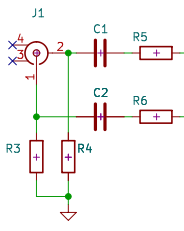
\includegraphics[keepaspectratio]{imgs/LTC_input.png}
				\end{figure}

	\subsection{GPI input circuit}\label{gpi-input-circuit}
		\paragraph{}GPI input circuit:
			\begin{figure}[!h] % Используйте [h] для размещения изображения "здесь"
				\centering
				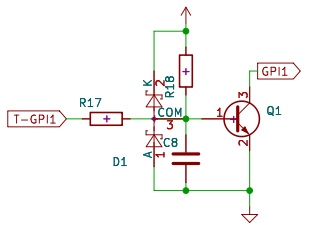
\includegraphics[keepaspectratio]{imgs/GPI_input.png}
				\caption{GPI Input Circuit}
				\label{fig:gpi-input}
			\end{figure}

	\subsection{GPO output circuit}\label{gpo-output-circuit}
		\paragraph{}GPO output circuit:
			\begin{figure}[!h] % Используйте [h] для размещения изображения "здесь"
				\centering
				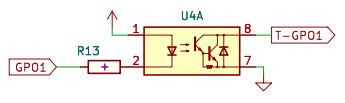
\includegraphics[keepaspectratio]{imgs/GPI_output.png}
				\caption{GPI Output Circuit}
				\label{fig:gpo-output}
			\end{figure}
	
	\subsection{USB 2.0 pinout}\label{usb-2.0-pinout}
		Connector 1 - J3 at Device.
		\begin{center}
			\begin{tabular}{|c|c|c|c|}
				\hline
				Connector 1 & Pin1 & Pin2 & Connector2 \\
				\hline
				DS1070-4 F & 1 & GND & USB-A 2.0 \\
				DS1070-4 F & 2 & D+ & USB-A 2.0 \\
				DS1070-4 F & 3 & D- & USB-A 2.0 \\
				DS1070-4 F & 4 & +5V & USB-A 2.0 \\
				\hline
			\end{tabular}
		\end{center}
	
	\section{Specifications}\label{specifications}
		
		\subsection{USB 2.0}\label{usb-2.0}
			\begin{itemize}
				\item
				Connector: USB-A 2.0 (via cable with HU-04 connector)
				\item
				19200 baud, no parity, 8 data bits, 1 stop bit.
			\end{itemize}
		
		\subsection{LTC input}\label{ltc-input-1}
			\begin{itemize}
				\item
				Balanced or unbalanced.
				\item
				Impedance: 10 kOhms.
				\item
				Level: 100mV p-p to 10V p-p.
				\item
				Speed: Nominal play @ 24, 25 30 frames per second.
			\end{itemize}
	
	\subsection{Power}\label{power}
		\begin{itemize}
			\item
			From USB 2.0.
			\item
			Load: Max 100 mA @ 5V.
		\end{itemize}
	
	\subsection{GPI Output}\label{gpi-output}
		\begin{itemize}
			\item
			Quantity 4.
			\item
			Drive: 10mA.
			\item
			Max. Reverse Voltage: 30V.
			\item
			True = transistor conducting.
		\end{itemize}
	
	\subsection{GPI Input}\label{gpi-input}
		\begin{itemize}
			\item
			Quantity 4.
			\item
			Internal pull up to logic Vcc.
			\item
			True = pull down to ground.
		\end{itemize}
	
	\subsection{Size/Weight}\label{sizeweight}
		\begin{itemize}
			\item
			83x67x20 mm .
			\item
			100 grams.
			\item
			Shipping weight 0.5 Kg.
		\end{itemize}
	
	\section{What's in the box}\label{whats-in-the-box}
		\begin{itemize}
			\item
			1 x LTC Reader with PCIe Low Profile IO Bracket
			\item
			1 x Cable HU-4 USB2.0 0.5m
		\end{itemize}
	
	\section{Revision Notes}\label{revision-notes}
	
	\section{Operational Hints}\label{operational-hints}
		LTC Reader will be restored to its stored settings if there is a power
		failure or momentary power drop out. It is advised that the desired
		settings be saved (see save settings command `SP\textgreater{}') to
		ensure that LTC Reader is in the desired mode, even after a power
		failure.
	
	\section{Ordering Information}\label{ordering-information}

		\begin{table}[h]
			\centering
			\resizebox{\textwidth}{!}{%
				\begin{tabular}{|c|l|}
					\hline
					Code & Description \\
					\hline
					LTC Reader & LTC Reader (1 x LTC input, 4 x GPI inputs, 4 x GPI outputs, USB 2.0), HU04-50 (Cable HU-4 to USB 2.0 50 cm long) \\
					PLS04-50 & Cable HU-4 to PLS-4 50 cm long \\
					HU04-50 & Cable HU-4 to USB 2.0 50 cm long (in box by default) \\
					\hline
				\end{tabular}%
			}
		\end{table}

	\section{How to contact us}\label{how-to-contact-us}
		Visit our website at \textbf{\href{http://www.simpletally.tv}{www.simpletally.tv}}
	
\end{document}
